\section{Discrete phase transitions}

During the whole course we have mainly focus on the description of physical systems behaves inside a particular phase, allowing us to understand which phase is stable at certain conditions. Nevertheless, another important question that we want to answer is how the transition to one phase to another happens exactly. We have talked, when we faced phase diagrams, how certain materials are able to go from one state to another in particular situation in a qualitative way, here we aim in describing it mathematically using the tools obtained from equilibrium Thermodynamics and kinetics.

The first thing that we shall say is that a phase transformation happens when, due to variation of certain parameters such as temperature or external field, the system breaks some internal symmetry finding more advantages to restructure itself in a more or less ordered way. For this reason, we are going to describe such phenomena using a set of parameters $\xi$ that mainly describes the order that is present inside the material, called \textbf{order parameters}. We have already seen some example of them in previous studies: like the long range order $\eta$ and the fractional density $X_i$ inside the study of the equilibrium inside a binary system. On a more general ground, during the study we will have to work with two main type of order parameters that we need to take into account, and we will define as follows.
\dfn{Conserved and Non-Conserved order parameters}
{
    An order parameter $\xi$ inside a system is conserved if it needs to be a constant inside a closed system, while non-conserved ones can change also if the system is closed.
}
\noindent
It's easy to understand that in the examples we have already seen $X_i$ is conserved, while $\eta$ is not. These two types of parameters highly influences how the transition behaves since the free energy will depend on them, $G(\xi)$, and based on their variation the energy landscape will be modified. To be more precise, we can evaluate a general form for the variation of free energy inside a material due to order parameters' changes in the two cases.
\thm{Variation for non-conserved $\xi$}
{
    Suppose that in a closed system composed of $N$ moles of material $n$ moles undergo a variation of a non-conserved order parameter from $\xi_1$ to $\xi_2$, where we assume $N\ll n$. The corresponding change of free energy of the whole system is
    \begin{equation}
        \delta G_u = n[G(\xi_2) - G(\xi_1)] \approx n G'(\xi_1)\delta\xi,
    \end{equation}
    where $G$ is the molar free energy of the material.
}
\pf{Proof}
{
    The proof is really simple since the order parameter is non-conserved it can change as wants inside the closed system, and so we can assume tha all the $N-n$ moles remains in $\xi_1$ being unperturbed by the change of the others. In this way we can set the change of free energy in the whole system as
    \begin{equation}
        \delta G_u = (N-n)G(\xi_1) + nG(\xi_2) - NG(\xi_1) = n[G(\xi_2) - G(\xi_1)].
    \end{equation}
    Also, the approximation with the first derivative is only the first order term of the Taylor series setting $\delta\xi \equiv \xi_2 - \xi_1$. 
}
\noindent
This shows how for non-conserved parameters the change totally relies only on the form of $G$ itself, with a behavior that is totally analogous to the one of the normal system. In the case of conserved parameters the thing changes a little becoming more interesting.
\thm{Variation for conserved $\xi$}
{
    Suppose that in a closed system composed of $N$ moles of material $n$ moles undergo a variation of a conserved order parameter from $\xi_1$ to $\xi_2$, where we assume $N\ll n$. The corresponding change of free energy of the whole system is
    \begin{equation}
        \label{eq:ConservedChange}
        \delta G_c = n\{G(\xi_2) - [G(\xi_1) + G'(\xi_1)(\xi_2 - \xi_1)]\} \approx \frac{n}{2} G''(\xi_1)\delta\xi^2,
    \end{equation}
    where $G$ is the molar free energy of the material.
}
\pf{Proof}
{
    In this case the total order parameter inside the material could not change, still $\xi$ can have local variation that can be compensated by the variation of the order parameter of the rest of the material. Meaning that, if $n$ moles now have $\xi_2$ as order parameter then all the remaining $N-n$ one's needs to have $\xi_1 - \Delta$ to compensate as follows 
    \begin{equation}
        (N-n)(\xi_1 + \Delta) +n\xi_1 = N\xi_1,
    \end{equation}
    which gives $\Delta = n(\xi_1 - \xi_2)/(N-n)$ so that $N\Delta \approx n(\xi_1 - \xi_2)$. In this way we can write down the following variation
    \begin{equation}
        \delta G_c = (N-n)G(\xi_1 + \Delta) + nG(\xi_2) - NG(\xi_1) \approx (N-n)[G(\xi_1) + G'(\xi_1)\Delta] + nG(\xi_2) - NG(\xi_1),
    \end{equation}
    which gives exactly what we wanted. Then, to have the approximation we can write $\xi_2 = \xi_1 + \delta\xi$ and expand the value of $G(\xi_2)$ to the second order obtain the final result.
}
\noindent
\begin{figure}[t]
    \centering
    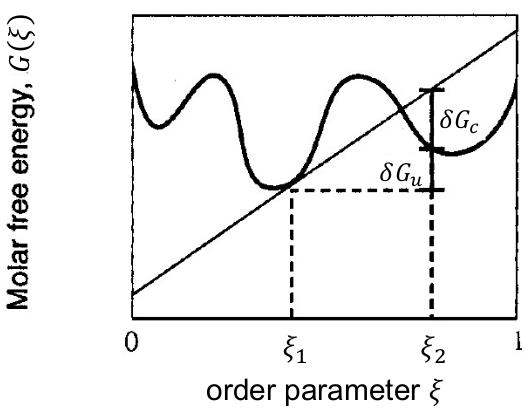
\includegraphics[width=0.4\textwidth]{Immagini/GVarXi.png}
    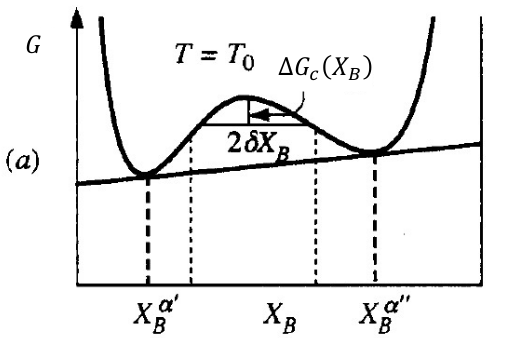
\includegraphics[width=0.45\textwidth]{Immagini/SpinodalPoints.png}
    \caption{
        Representation of a free energy landscape depending on order parameters with the opportune variations on the left, and a representation of a $G(X)$ with the spinodal points in evidence on the right.
    }
    \label{fig:FirstPhaseTrans}
\end{figure}
In this case the variation of the free energy do not simply depend on the form of $G$ but also on the convexity of it. In particular, the variation of free energy due to order changes is mainly given by the second derivative. Meaning that if we are in a local maximum $G'' < 0$ and the system is \textbf{unstable} wanting to change to a minimum where $G'' > 0$ so that even if $\xi$ changes the variation of energy is positive and the system is so \textbf{metastable}. Where we use the word metastable and not stable since it's not sad that the system will remain in that minimum forever, due to large variation of energy coming external factors, like thermal fluctuations, the system can jump to another valley and sit there for some time until another jump happens.

This description of how $G$ changes due to order parameters is really general and profound, showing us not only how the free energy changes based on the nature on the parameter itself, but also suggest to us how that change happens. Let's focus a moment on \eqref{eq:ConservedChange} in the situation depicted on \figref{fig:FirstPhaseTrans}, the system will have two metastable state divided by an energy barrier which defines an unstable region. In particular, the unstable region is delimited by the $\xi$ so that $G''(\xi) = 0$, where $X_B$ is the order parameter in that case. We have already talk about points with such a property calling them \textbf{spinodal points}, basically the region inside the spinodal points is unstable meaning that it will natural evolve continuously to a minimum. Then, when it reaches a metastable position it will sit there and remain there until a sudden discontinuous change happens, and the system changes minimum to sit in. These two different behaviors define the two main types of phase transitions that we are going to touch called \textbf{continuous} and \textbf{discontinuous} phase transitions, which mainly differ in how quick the change happens and in the extension of the change, having that discontinuous transformations are usually locals while continuous are more global. 

In this first section we will focus first on the discontinuous type describing the main, and simpler, possible forms of such transitions: like the formation of a water droplet in clouds. We will leave the continuous case to a further section.

\subsection{Nucleation theory}

Nucleation is an important phenomenon that consist in the spontaneous formation of cluster of components inside the material that will then grow over time through different mechanisms like coarsening. In particular, in the classical theory of nucleation the system goes through four different steps: an initial incubation where no cluster are formed over time, to then a steady-state situation where the number increase in time reaching a maxima where driving forces of nucleation start to reduce, and then the coarsening that will decrease the number generating bigger grains. Inside such a complex kinetic behavior we aim first in the description of the distribution of cluster inside cluster space $N_\nu(t)$, where $N_\nu$ is the number of cluster possessing $\nu$ monomers components inside them.

To start the study we can try to write down a form for the variation of free energy of the system in the formation of a cluster with $\nu$ components. We can assume that inside a matrix in state $\alpha$ and chemical potential for component $\mu^\alpha$ start to grow a cluster in state $\beta$ which changes also the chemical potential of the $\nu$ monomers. Such a formation will so generate a simple variation of free energy to which we will need also to add the energy coming from the interface $\gamma A$, where $A \propto V^{2/3}$ and $V \propto \nu$, meaning that naming $\eta$ the constant of proportionality we have
\begin{equation}
    \Delta G_\nu = \nu\left( \mu^\beta - \mu^\alpha \right) + \eta\nu^{2/3}\gamma.
\end{equation}
\begin{figure}[t]
    \centering
    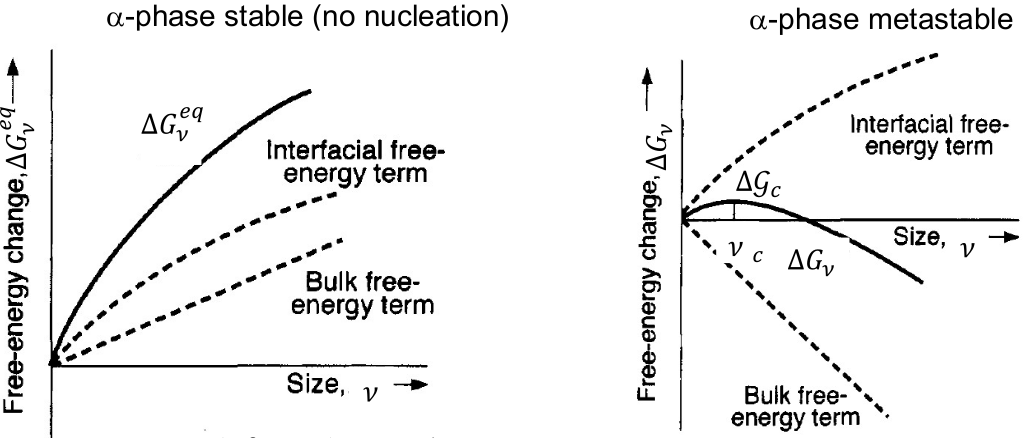
\includegraphics[width=0.8\textwidth]{Immagini/FreeEnNucle.png}
    \caption
    {
        Graph of the variation of free energy due to nucleation as a function of cluster size, in particular on the left there's the case where the chemical potential of the $\alpha$ matrix phase is more favorable than the one of the $\beta$ grain phase, and on the right the opposite.
    }
    \label{fig:FreeEnNucle}
\end{figure} 
It's form can be seen in \figref{fig:FreeEnNucle}, where we can see clearly how the starting bulk term completely determine the possibility of nucleation. In fact, when $\nu$ is small the term that leads the change in free energy is the surface one, which is always positive, meaning that cluster of small size will always be energetically unfavorable, while as $\nu$ increase $\mu^\beta - \mu^\alpha$ will start to lead. In this way we can understand that, if the difference in the chemical potential is negative, cluster starts to grow consistently only when they reach a certain critical value from which $\Delta G_\nu$ starts to decrease
\begin{align}
    &\eval{\dv{\Delta G_\nu}{\nu}}_{\nu = \nu_c} = 0, &\nu_c = -\left( \frac{2\eta\gamma}{3(\mu^\beta - \mu^\alpha)} \right)^3.
\end{align}
Therefore, we will have that in a first moment the cluster are not able to form for a long period of time due to the increase in free energy, but there is still a probability that due to thermal fluctuations, or other external factor, one cluster of size $\nu_c$ forms starting increasing its size naturally from there and forming the center of nucleation. Meaning that we are already able to understand the presence of the \textbf{incubation phase}, which can be overcome through probability fluctuations typical of a discontinuous phase transformation.

We can now start to model the process of formation of the grains overtime, and in order to do that we want to work inside the space of cluster size $N_\nu$. Meaning that we want to find out a form for the flux $J_\nu(t)$ describing how many cluster goes at certain time from having $\nu$ components to $\nu+1$. Such a quantity can be easily modelled by assuming that the probability of one monomer to enter the cluster over time is $\beta_\nu$, while the probability for one to hoop out of it is $\alpha_\nu$ having that
\begin{equation}
    J_\nu(t) = \beta_\nu N_\nu(t) - \alpha_{\nu+1} N_{\nu+1}(t).
\end{equation}
Using such a description allows us to find out some important information on the form of the distribution itself. For example, we can see what happens in a case where the system reaches an equilibrium, assuming that the $\alpha$ phase is stable, $\mu^\beta - \mu^\alpha > 0$, we can find out the following.
\thm{Equilibrium distribution}
{
    When the matrix $\alpha$ phase is stable respect to the grain $\beta$ one the system will evolve in time reaching an equilibrium where, still, a series of clusters are formed following the distribution given by
    \begin{equation}
        N_\nu^{eq} = N\exp\left( -\frac{\Delta G_\nu}{k_BT} \right),
    \end{equation}
    with $N$ the total number of atoms.
}
\pf{Proof}
{
    This demonstration was not done during the lectures.
}
\noindent
Such a result is really helpful for us since allows for the creation of a relation between the different probabilities $\alpha_\nu$ and $\beta_\nu$ defined earlier. In fact, we can say that at equilibrium $J_\nu = 0$ for every value of $\nu$ and so the following is true
\begin{equation}
    \label{eq:CoeffRelation}
    \beta_{\nu + 1} = \beta_\nu\frac{N_\nu}{N_{\nu+1}} = \beta_\nu\exp\left( -\frac{\Delta G_{\nu+1} - \Delta G_\nu}{k_BT} \right).
\end{equation}
Still, such a distribution is not the one we are more interested in, in fact inside such an equilibrium distribution we have only the formation of small clusters due to fluctuations inside the material, the number larger cluster is zero inside such a quick descending distribution. The situation in the case where the $\alpha$ phase is metastable, with $\mu^\beta - \mu^\alpha < 0$, the situation changes since the system will undergo an irreversible transformation that through the stable phase that involves nucleation. Meaning that the final goal is to find out a way to describe the non-equilibrium distribution of clusters $Z_\nu(t)$, in particular focussing on the form of $J_\nu$ still defined as before in a steady state situation.
\thm{Non-equilibrium steady-state flux}
{
    When the matrix $\alpha$ phase of the material is metastable the system will undergo a nucleation that, passed the state of incubation, will grow in a steady state regime given by the flux in cluster size space $J$ as
    \begin{equation}
        \label{eq:SteadyStateFlux}
        J = N\beta_c \sqrt{\frac{\Delta G_c}{3\pi k_BT\nu_c^2}}\exp\left( -\frac{\Delta G_c}{k_BT} \right),
    \end{equation}
    where $\beta_c$ is the probability of capture by the critical size cluster.
}
\begin{figure}[t]
    \centering
    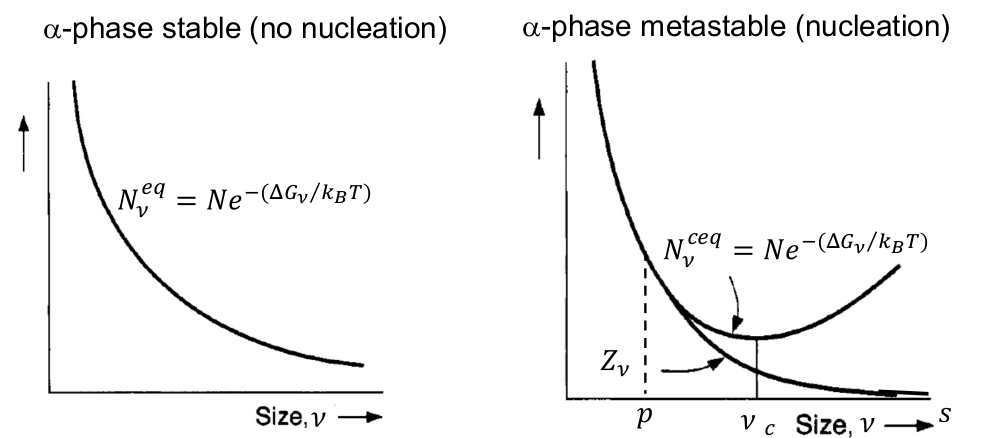
\includegraphics[width=0.8\textwidth]{Immagini/DistributionsGrains.png}
    \caption
    {
        Plot of the equilibrium and non equilibrium distribution in the two cases where $\alpha$ is stable and metastable in order to guide better the demonstration of the results.
    }
    \label{fig:DistributionsGrains}
\end{figure}
\pf{Proof}
{
    During such a demonstration we will assume the condition of constrained equilibrium allowing for the relation between the coefficients in \eqref{eq:CoeffRelation} to be valid also in this particular case\footnote{Probably better to look up on the internet for such a piece of theory.}. This allows us to write down that
    \begin{equation}
        J_\nu = \beta_\nu Z_\nu - \alpha_{\nu+1} Z_{\nu+1} = \beta_\nu N_\nu^{eq}\left( \frac{Z_\nu}{N_\nu^{eq}} - \frac{Z_{\nu+1}}{N^{eq}_{\nu+1}} \right),
    \end{equation}
    then we can recall that in a steady-state situation we have $J_\nu = J_\omega$ for every $\nu$ and $\omega$, so that $J_\nu = J$. Then we will also assume that for small $\nu$ also in $Z_\nu$ the leading term will be the one given by the surface energy, which do not change from equilibrium and non-equilibrium case, meaning that the distribution remains the same. While for larger sizes the distribution needs to drop respect to what $N^{eq}$ predict, since the exponent would have a positive term inside after $\nu_c$, having that we assume the form
    \begin{equation}
        Z_\nu = 
        \begin{cases}
            N_\nu & \nu \le p < \nu_c\\
            0 & \nu \ge s > \nu_c
        \end{cases}.
    \end{equation}
    Where $p$ and $s$ are integer values chosen in order for $Z_\nu$ to fit better to the equilibrium distribution as in \figref{fig:DistributionsGrains}. In this situation we can write down the following thing
    \begin{equation}
        \frac{J}{\beta_\nu N_\nu} = \left( \frac{Z_\nu}{N_\nu^{eq}} - \frac{Z_{\nu+1}}{N^{eq}_{\nu+1}} \right),
    \end{equation}
    which can be summed up over all the possible grain sizes in order to obtain a telescopic series
    \begin{equation}
        \sum_{\nu=p}^s \frac{J}{\beta_\nu N_\nu} = \frac{Z_p}{N_p} - \frac{Z_{s+1}}{N_{s+1}} = 1,
    \end{equation}
    since $Z_{s+1} = 0$ and $Z_p = N_p$. Therefore, we can write a simple form for $J$ as a summation that can be approximated remembering that $\beta_\nu$ needs to have a maximum at $\nu_c$ since is the size at which caching becomes favorable
    \begin{equation}
        J = \left[ \sum_{\nu=p}^s \frac{1}{\beta_\nu N_\nu} \right]^{-1} \approx \left[ \frac{1}{\beta_c N}\sum_{\nu=p}^s e^{\Delta G_\nu/k_BT} \right]^{-1}.
    \end{equation}
    In this situation we can approximate the sum for an integral and also expand $\Delta G_\nu$ around $\nu_c$ since is its maximum and the main contribution is near there, having
    \begin{align}
        &\Delta G_\nu \approx \Delta G_c + \frac{(\nu - \nu_c)^2}{2}\eval{\pdv[2]{\Delta G_\nu}{\nu}}_{\nu = \nu_c} &\eval{\pdv[2]{\Delta G_\nu}{\nu}}_{\nu = \nu_c} = -\frac{2}{9}\eta\gamma\nu_c^{-4/3} = -\frac{2}{3}\frac{\Delta G_c}{\nu_c^2}.
    \end{align}
    Then we can simply insert inside the summation and integrate as
    \begin{equation}
        \sum_{\nu=p}^s e^{\Delta G_\nu/k_BT} \approx e^{\Delta G_{c}/k_BT} \int_p^s \dd \nu \exp\left( -\frac{2}{3}\frac{\Delta G_c}{\nu_c^2k_BT}\frac{(\nu - \nu_c)^2}{2} \right) \approx e^{\Delta G_{c}/k_BT}\sqrt{\frac{3\pi k_BT\nu_c^2}{\Delta G_c}},
    \end{equation}
    where we have expanded the extreme of the Gaussian integral to cover the whole domain since the tails give a small contribution. Then by inserting such result inside the form of $J$ we obtain the wanted result.
}
\noindent
Now, this is an interesting result that describes the evolution of the nucleation inside the material in the \textbf{steady-state phase} where the number of cluster with greater size increase linearly in time since $J$ is constant. Also, we can see how inside $J$ all the contribution are given by $\nu_c$, since is effectively the most important term, but still the factor $\sqrt{\bullet}$, called \textbf{Zeldovich factor}, is giving us corrections to consider also the surrounding contribution. In fact, if we didn't expand $\Delta G_\nu$ to first order but zeroth we will have had a $1$ in its place, instead a number $\sim 0.1$ is given. At last, we shall understand that the only term that we don't know how to write down inside $J$ is the form of $\beta_c$, which still can be described using a series of model resumed shortly inside the slides.

Before going into the next topic, we shall first make some remarks for the result that we have obtained right now. In particular, we shall say that the nucleation that we have described is generally called \textbf{homogeneous nucleation} and is characterized by the creation of the clusters out of atmosphere with no preferential position on where to appear. In this type of nucleation the result \eqref{eq:SteadyStateFlux} is telling us a lot on the velocity of the process, and its value depends strongly on $\Delta G_c$ giving us the following insights
\begin{enumerate}[label*=\protect\fbox{\arabic{enumi}}]
    \item $\Delta G_c \propto \gamma^3$ and in incoherent interfaces $\gamma \approx \SI{0.5}{Jm^{-2}}$, while in coherent is lower by at least a factor of three. Therefore, in most situations homogeneous nucleation is possible only for coherent interfaces;
    \item $\Delta G_c \propto (\mu^\beta - \mu^\alpha)^{-2}$ shows how $J$ can increase suddenly due to temperature variations that modify the driving force;
    \item One can estimate the value of $\Delta G_c$ to have an idea by using $J\approx \SI{1}{cm^{-3}s^{-1}}$ along with $\beta_c \approx 10^12$ and a Zeldovich factor of $0.1$ to find $\Delta G_c \approx 76k_BT$;
    \item In the case of solid-solid nucleation we shall include inside the free energy also a strain term that is often described using the volumetric density of bulk free energy $\Delta g_B$. Basically, to the normal energy of the bulk inside the system a $\Delta g_\epsilon$ term due to the strain caused by the generation of solid clusters inside a solid appears, a term that can be neglected if the nucleation happens inside a liquid or a gas for obvious reasons.
\end{enumerate}
Such information can be important in the study of the phenomena in a general way, in particular we shall remember the notion of volumetric density of free energy $\Delta g$ since we are going to use it in future topics.

\ex{CNT-Exercise}
{
    At the end of the topic the prof showed a really simple exercise to understand how much the steady-state flux depends on the free energy seeing how also small variations can cause rapid increases. The assumption is that in a system with an atomic fraction of $B$ atoms of $X_B = 0.3$ homogenized at $\SI{1200}{K}$ and quenched to $\SI{800}{K}$ has a $\beta$-phase nucleation rate of $\SI{e6}{m^{-3}s^{-1}}$. We want to increase the density of $B$ atoms in order to bring the flux at $\SI{e21}{m^{-3}s^{-1}}$ knowing that
    \begin{align}
        &\Delta g_B = [-100(X_B - 0.3) - 9]10^{7}\si{Jm^{-3}}, &\gamma = \SI{75}{Jm^{-2}}.
    \end{align}
    We can so write down the total variation of free energy of the system by using the following equation
    \begin{equation}
        \Delta G = \frac{4\pi}{3}r^3\Delta g_B + 4\pi r^2 \gamma,
    \end{equation}
    which can be maximized to found out $\Delta G_c$ at the value of
    \begin{align}
        &r_c = -2\frac{\gamma}{\Delta g_B}, &\Delta G_c = \frac{16\pi}{3}\frac{\gamma^3}{\Delta g_B^2}.
    \end{align}
    Knowing that we can insert everything in the known formula for $J$ and find out that in order to increase the flux by $15$ orders of magnitude we only need to increase $X_B$ by a $0.03$, so that $\Delta G_c$ becomes half.
}

\subsection{Heterogeneous nucleation}

The next important case that we shall address is the case where the nucleation happens in some preferential points inside the system generating \textbf{Heterogeneous nucleation}. In particular, we will focus on the case where the cluster prefer to form in the interface's region, meaning that a surface is already present and so the formation of the grain can be more favorable due to variations of surface free energy. We will not go into the theoretical treatment of this particular phenomenon, but still we will need to address two cases: the creation of clusters in a grain boundary, where a solid-solid interface is present, and the film deposition, where the interface where the grain forms is a solid-gas one.

In the first case we can have that the clustering begins in the interface between two solid phases $\alpha$ generating a grain that changes the free energy thanks to the variation of chemical potential of the grain's $\beta$ phase and the interface free energy variation. In the case without grain in the middle the interface posses an energy that is given by $\gamma^{\alpha\alpha}$, but it's possible that the $\alpha-\beta$ interface has a better surface free energy $\gamma^{\alpha\beta}$ having that the formation of clusters to substitute the $\alpha-\alpha$ interface is really favorable.
\begin{figure}[b]
    \centering
    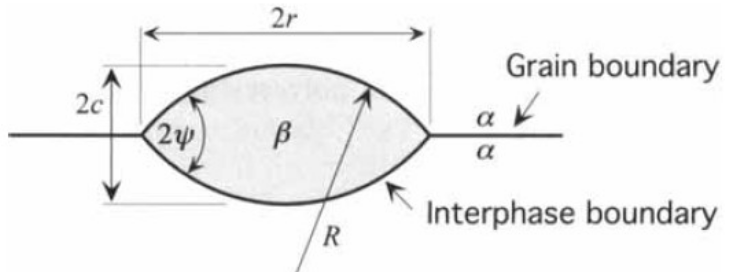
\includegraphics[width=0.8\textwidth]{Immagini/SolidSolidInter.png}
    \caption{
        Representation of a heterogeneous nucleation in the solid-solid interface, important to see how the cluster formed takes the shape of a lens with an angle that depends on the surface tensions.
    }
    \label{fig:SolidSolidInter}
\end{figure}
Also, the shape that the cluster will take depends on how favorable such substitution is, giving a general form of a lens as in \figref{fig:SolidSolidInter} with the angle given by a known result.
\newpage
\thm{Young's equation solid-solid}
{
    The shape of a grain in a solid-solid interface is defined by $\gamma^{\alpha\alpha}$ and $\gamma^{\alpha\beta}$ and is given by
    \begin{equation}
        \label{eq:YoungEqua}
        \gamma^{\alpha\alpha} = \gamma^{\alpha\beta}\cos\psi.
    \end{equation}
}
\noindent
Where one can grasp a lot of information, for example if $\gamma^{\alpha\alpha} = 0$ means that we don't have the interface at all not having heterogeneous nucleation at all with $\psi = \pi/2$ so that the grain are spherical as in the homogeneous case. Instead, if $\gamma^{\alpha\alpha} = 2\gamma^{\alpha\beta}$ the angle is flat meaning that the interface catalyze the reaction so well that a continuous film around the interface is created. Also, we can evaluate the increase in free energy that such a grain can generate in the system by looking at the following result.
\thm{Grain free energy solid-solid}
{
    If a nucleation starts on a solid-solid interface the increase of free energy of the system takes the form
    \begin{equation}
        \Delta G^{GB} = \left( \frac{2\pi R}{3}\Delta g_B + 2\pi R^2\gamma^{\alpha\beta} \right)\left( 2 - 3\cos\psi + \cos^3\psi \right).
    \end{equation}
}
\pf{Proof}
{
    We can proof it by using that fact that the volume and the area of the lens figure formed can be computed using
    \begin{align}
        &V = \frac{2\pi R}{3}( 2 - 3\cos\psi + \cos^3\psi ), &A = 4\pi R^2(1- \cos\psi),
    \end{align}
    where $R$ is the radius of the grain. Then we can evaluate the variation of energy due to the creation of a $\beta$ bulk and the increase of the interface along with the elimination of the $\alpha-\alpha$ one as
    \begin{equation}
        \Delta G^{GB} = V\Delta g_B + A\gamma^{\alpha\beta} - \pi r^2\gamma^{\alpha\alpha},
    \end{equation}
    then we can use the fact that $r \approx R\sin\psi$ along with Young's equation to obtain the final result.
}
\noindent
One can see how such a form is similar to the one of the homogeneous case, having that we can see that the first term is exactly equal to $1/2$ the homogeneous energy while the angular term is what really defines if the heterogeneous nucleation is preferred or not. Such a term is also called \textbf{wetting factor}, and we can see how the following is true
\begin{equation}
    \frac{\Delta G_c^{GB}}{\Delta G_c^H} = \frac{1}{2}\left( 2 - 3\cos\psi + \cos^3\psi \right),
\end{equation}
this term shows how the energy is basically always less in the heterogeneous case, in fact one can see how since $\gamma > 0$ the wetting term is always contained in $[0, 1]$. Meaning that the nucleation phenomena is generally more favorable at the grain boundaries and becomes analogous at the homogeneous case only if the interface is coherent, as we have already anticipated previously. At last, it's possible to give an estimate of the steady-state rate of growth of the heterogeneous nucleation by using the homogeneous result and the density of boundary sites  as follows
\begin{align}
    &n^{GB} = n\frac{\delta}{D} &\frac{J^{GB}}{J^H} = \frac{n^{GB}}{n}\exp\left[ -\frac{\Delta G_c^{GB} - \Delta G_c^H}{k_BT} \right],
\end{align}
where $\delta$ is the grain boundary thickness and $D$ the average grain diameter.

Now we can work with the case where the growth happens in a solid-gas interface, in this situation what happens is that three different surface free energies appears, since also the interface formed by the cluster and the gas will have a specific $\gamma$. In this situation is also possible to predict the form of the generated cluster that is given by the form seen in \figref{fig:SolidGasInterf},
\begin{figure}
    \centering
    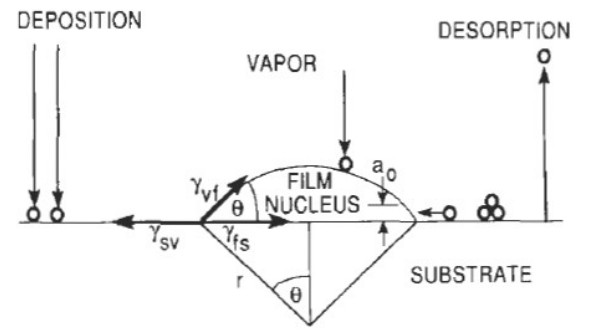
\includegraphics[width=0.8\textwidth]{Immagini/SolidGasInterf.png}
    \caption{
        Representation of the nucleation on a solid-gas interface showing how the cluster formed is elongated due to surface effect generating a more uniform film.
    }
    \label{fig:SolidGasInterf}
\end{figure}
where we can see how the different surface tensions generate forces due to Marangoni effect giving at the cluster a more homogeneous form. The latter can be, once again, described using a clever result that connects the angle $\theta$ to surface tensions.
\thm{Young's equation solid-gas}
{
    The shape of the cluster on a solid-gas interface is defined by the three surface tensions inside the system and is given by
    \begin{equation}
        \gamma^{sv} = \gamma^{fs} + \gamma^{vf}\cos\theta.
    \end{equation}
}
\noindent
Knowing that, we can have a look at how the cluster will look like in various cases. For example, if $\gamma^{sv} < \gamma^{fs} + \gamma^{vf}$ then the angle is greater than zero, so the atoms on the surface are more attracted to each other than the substrate forming various islands with same form. Instead, if the surface tensions are equal the angle is null giving out that the atoms prefer to attach to the substrate forming a perfect layer that grows homogeneously, also in autoepitaxy we set $\gamma^{fs} = 0$. At last, the case where $\gamma^{sv} > \gamma^{fs} + \gamma^{vf}$ posses a behavior similar to the one before generating a homogeneous film, but the strain energy increase as the layer growth giving rise to phenomena of strain release by separation in island during the growth. Then, to complete the analogy to the previous case we can have a look to the free energy change inside the system due to the cluster formation.
\thm{Grain free energy solid-solid}
{
    If a nucleation starts on a solid-gas interface the increase of free energy at the critical size of the system takes the form
    \begin{equation}
        \Delta G_c = \frac{16\pi\gamma_{vf}^3}{3\Delta g_B^2}\frac{2- 3\cos\theta + \cos^3\theta}{4}.
    \end{equation}
}
\pf{Proof}
{
    One can compute the total energy change that comes from the cluster by using the same approach as before obtaining
    \begin{equation}
        \Delta G = \pi(2 - 3\cos\theta + \cos^3\theta)\left( \frac{r^3\Delta g_B}{3} + r^2\gamma^{vf} \right),
    \end{equation}
    then we can maximize it and obtain the final result.
}
\noindent
Once again one can see how this value is equal to the homogeneous nucleation one multiplied by a wetting factor that is always less than unity. Meaning that, again, the creation of nuclei inside a system is more favorable near an interface.

\nt
{
    The fact that clusterization is more favorable near interfaces is an important fact in experimental techniques, in fact a lot of methods utilize them to achieve results. The simplest example is the physical vapor deposition, where a homogeneous thin film of material is constructed on a substrate inside a high vacuum chamber by vaporize a material so that the atoms from it travels in vacuum deposit on the surface of the substrate. In this way, by using the right materials, we can construct the film as described by the nucleation on solid-gas interface.
}